\chapter{Executive Summary}
\label{ch:fdsp-execsum}

\section{Introduction}
\label{sec:fdsp-exec-introduction}
%Broad physics motivation for the detector.


The overriding physics goals of \dword{dune} are the search for leptonic \dword{cp} violation, the observation of neutrino bursts from supernovae, and the search for nucleon decay as a signature of a Grand Unified Theory underlying the Standard Model. Central to achieving this physics program is the construction of a detector that combines the many-kiloton fiducial mass necessary for rare event searches with sub-centimeter spacial resolution in its ability to image those events, allowing us to identify the signatures of the physics processes we seek among the numerous backgrounds. The \dword{sp} \dword{lartpc}~\cite{Rubbia:1977zz} allows us to achieve these dual goals, providing a way to read out with sub-centimeter granularity the patterns of ionization in $\SI{10}{kt}$ volumes of liquid argon resulting from the $O(\SI{1}{MeV})$ interactions of solar and supernova neutrinos up to the $O(\SI{1}{GeV})$ interactions of neutrinos from the \dword{lbnf} beam.

To search for leptonic \dword{cp} violation, we must search for \nue appearance in the \dword{lbnf} \numu beam. This requires the ability to separate electromagnetic activity induced by charged-current \nue interactions from similar activity arising from photons, for example, those from $\pi^{0}$ decay. Two signatures allow this: photon showers are preceded by a gap prior to the conversion of the photon, characterized by the \SI{14}{cm} conversion length; and the initial part of a photon shower has twice the $\mathrm{d}E/\mathrm{d}x$ of an electron-induced shower, clearly measurable given the signal-to-noise requirements on our ability to measure the ionization of the argon. To search for proton decay, where the primary channel of interest is $p\rightarrow K^{+}\overline{\nu}$, we must identify kaon tracks as short as a few centimeters, which can be done thanks to the sub-\si{cm} spacial resolution of the \dword{lartpc}. It is also vital to accurately fiducialize these proton-decay events to suppress cosmic-muon-induced backgrounds, and here the detection of argon-scintillation photons is important. Detecting supernova neutrino bursts poses different challenges: those of data-rate and detector reliability. To fully reconstruct a supernova burst, the entire detector must be read out, at up to $\SI{2}{\tera\byte/\second}$, for \SIrange{30}{100}{s}, including a $\sim\!\SI{4}{s}$ pre-trigger window. And to ensure these rare events are not missed, all detector sub-systems must work together to ensure the highest live-time possible.

In what follows, we give an overview of the basic operating principles of a \dword{sp} \dword{lartpc}, followed by a description of the \dword{dune} implementation. We then discuss each of the sub-systems separately, connecting the high-level design requirements and decisions to the overriding physics goals of \dword{dune}.

\section{The Single Phase Liquid Argon Time Projection Chamber}
\label{sec:fdsp-exec-splar}
%General operating principle

\begin{dunefigure}[The single-phase liquid-argon time-projection chamber]{fig:LArTPC}
{The general operating principle of the single-phase liquid-argon time-projection chamber.}
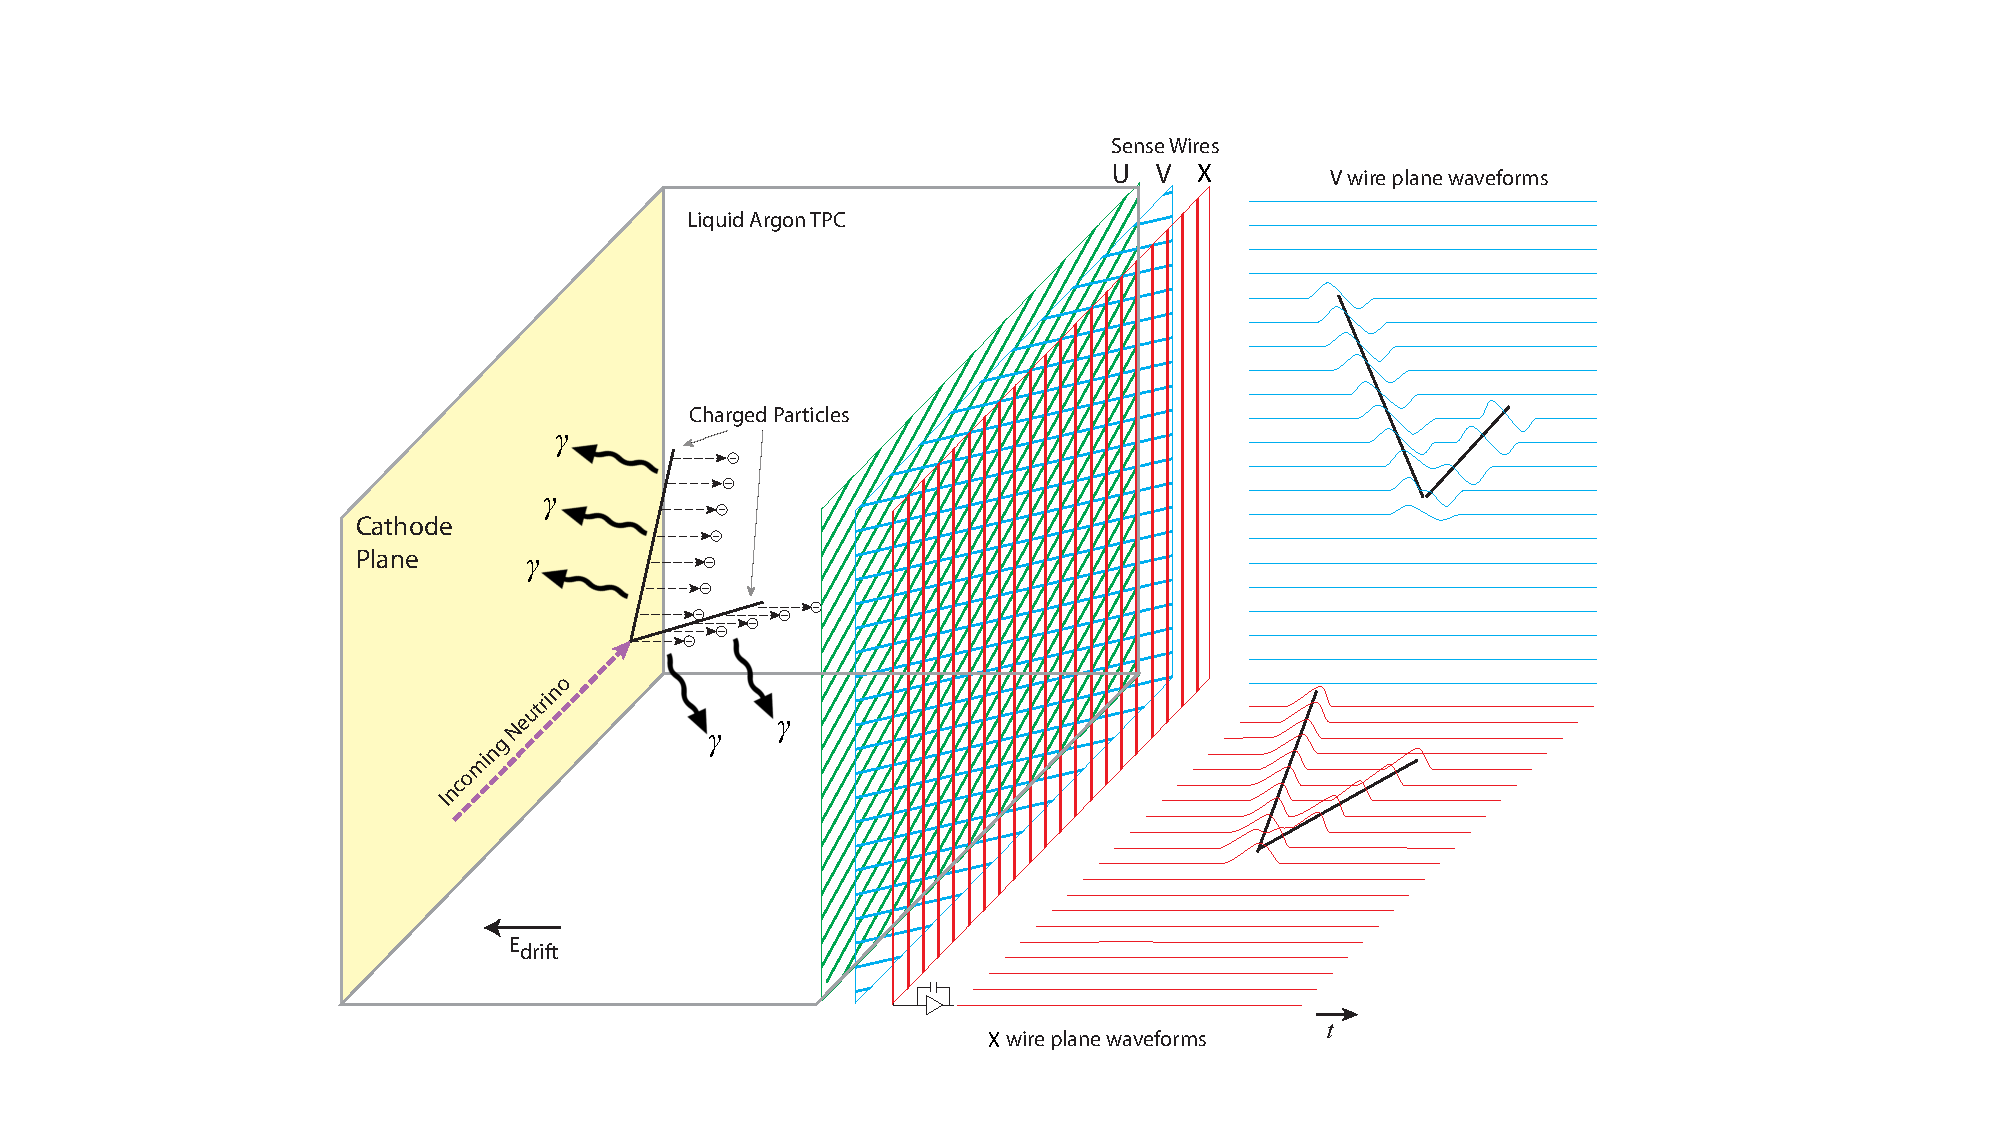
\includegraphics[trim={5cm 0 5cm 0},clip,width=0.8\textwidth]{graphics/TheBoPicture.pdf}
\end{dunefigure}

Figure~\ref{fig:LArTPC} shows the general operating principle of a \dword{sp} \dword{lartpc}, as has been previously demonstrated by \fixme{I don't have a dword for ICARUS. All the others are in the common glossary.} ICARUS~\cite{Icarus-T600}, \dword{microboone}~\cite{microboone}, \dword{argoneut}~\cite{Anderson:2012vc}, \dword{lariat}~\cite{Cavanna:2014iqa}, and \dword{protodune}~\cite{Abi:2017aow}. A large volume of liquid argon is subjected to a strong electric field of a few hundred volts per centimeter. Charged particles passing through the detector ionize the argon, and the ionization electrons drift in the electric field to the anodic wall over $O(\SI{100}{\micro\second})$. This anode consists of three layers of active wires forming a grid. The relative voltage between the layers is chosen to ensure the first two layers are transparent to the drifting electrons, and these layers produce bipolar induction signals as the electrons pass through them. The final layer collects the drifting electrons, resulting in a monopolar signal.

Liquid argon is also an excellent scintillator, at \SI{126.8}{\nano\meter}, and this fast scintillation light, once shifted into the visible, is collected by photon-detectors placed either in or near the anode plane. The photon detectors provide a $t_{0}$ for every event, telling us when the ionization electrons begin to drift. Relative to this $t_{0}$, the time at which the ionization signal reaches the anode allows reconstruction of the event topology in the drift coordinate; the precision of this $t_{0}$, therefore, directly corresponds to the precision of the spacial reconstruction in this direction. In addition to our ability to reconstruct topologies in the drift direction, this $t_{0}$ precision defines our ability to fiducialize proton-decay events and our ability to apply drift corrections to the ionization charge.

The pattern of ionization collected on the grid of anode wires provides the reconstruction in the remaining two coordinates perpendicular to the drift direction. A closer spacing of the wires, therefore, results in better spacial resolution, but, in addition to increasing the cost of the readout electronics due to the additional wire channels, a closer spacing worsens the signal-to-noise of the ionization measurement because the same amount of ionization charge is now divided over more channels. Signal-to-noise is an important consideration because the measurement of the ionization collected is a direct measurement of the $\mathrm{d}E/\mathrm{d}x$ of the charged particles, which is what allows us to perform both calorimetry and particle identification.

\section{The \dword{dune} Single Phase Far Detector Module}
\label{sec:fdsp-exec-dunefd}
%Explain 10 kt modules, and then explain the overall setup.
%As part of this, explain the main design parameters and how they relate to the physics drivers.

\begin{dunefigure}[A $\SI{10}{\kilo\tonne}$ DUNE Far Detector single-phase module.]{fig:DUNESchematic}
{A $\SI{10}{\kilo\tonne}$ DUNE Far Detector single-phase module, showing alternating anode (A) and cathode (C) planes.}
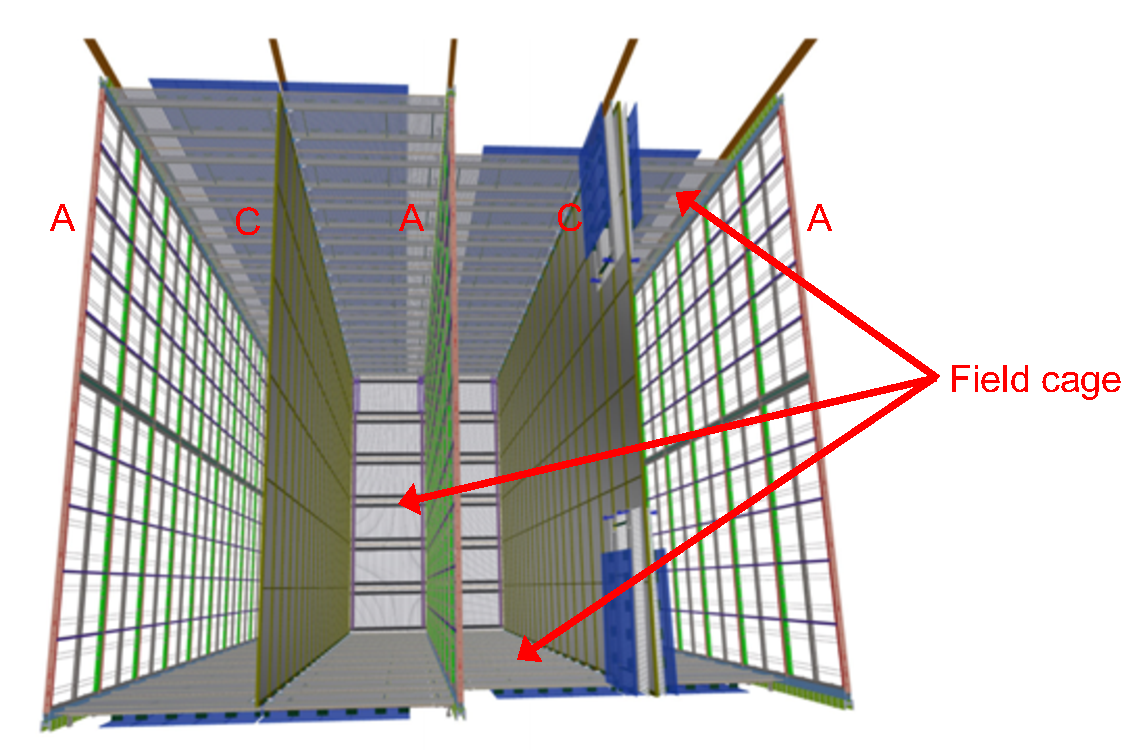
\includegraphics[width=0.8\textwidth]{DUNESchematic.pdf}
\end{dunefigure}

The DUNE \dword{sp} \dword{lartpc} consists of \SI{10}{\kilo\tonne} modules, contributing to the full \SI{40}{\kilo\tonne} \dword{fd} fiducial mass. Figure~\ref{fig:DUNESchematic} shows a \SI{10}{\kilo\tonne} module. Inside a cryostat of outer dimensions $62\times 19\times \SI{18}{\meter^{3}}$, four $\SI{3.5}{\meter}$ drift volumes are created between five alternating anodic and cathodic walls, each wall having dimensions of $\SI{58}{\meter}\times \SI{12}{\meter}$.

Each cathodic wall in a module is called a \dword{cpa} array. The \dword{cpa} is the $\SI{1.2}{\meter}\times\SI{4}{\meter}$ panel from which the \dword{cpa} arrays are formed; each \dword{cpa} array contains $150$ \dword{cpa} units. These \dword{cpa} arrays are held at $-\SI{180}{\kilo\volt}$. With the anodic walls held close to ground, this results in a \SI{500}{\volt/\centi\meter} drop across the drift volume. A \dword{fc} surrounds the remaining open sides of the \dword{tpc}, ensuring the field is uniform to at least 1\% throughout the active volume. A typical minimum ionizing particle passing through the argon produces around $60k$ ionization electrons per centimeter, and these drift towards the anodes at around $\SI{1.5}{\mm/\micro\second}$; the time taken to drift the full distance from cathode to anode would therefore be around $\SI{2.4}{\milli\second}$.

The anode walls are each made up of 150 \dword{apa}s that are $\SI{6}{\meter}\times\SI{2.3}{\meter}$ in dimension. As shown in Figure~\ref{fig:APAStack}. the \dword{apa}s hang vertically, and each anode wall is two \dword{apa}s high; the bottom \dword{apa} hangs from the \dword{apa} above it. The \dword{apa}s are two-sided, with the three active wire layers and an additional shielding layer wrapped around them. The collection layer is called the $x$-layer; the induction layer immediately next to that is called the $v$-layer; the next induction layer is the $u$-layer; and the shielding layer is the $g$-layer. $x$-layer and $g$-layer wires are vertical; the $u$- and $v$-layer wires are at \SI{35.7}{\degree} to the vertical.

\begin{dunefigure}[A stack of two anode plane assemblies.]{fig:APAStack}
{Left: two \dword{apa}s hanging above each other. Right: a zoom into the top and bottom ends of the \dword{apa} stack showing the readout electronics, and the centre of the stack where the \dword{apa}s meet.}
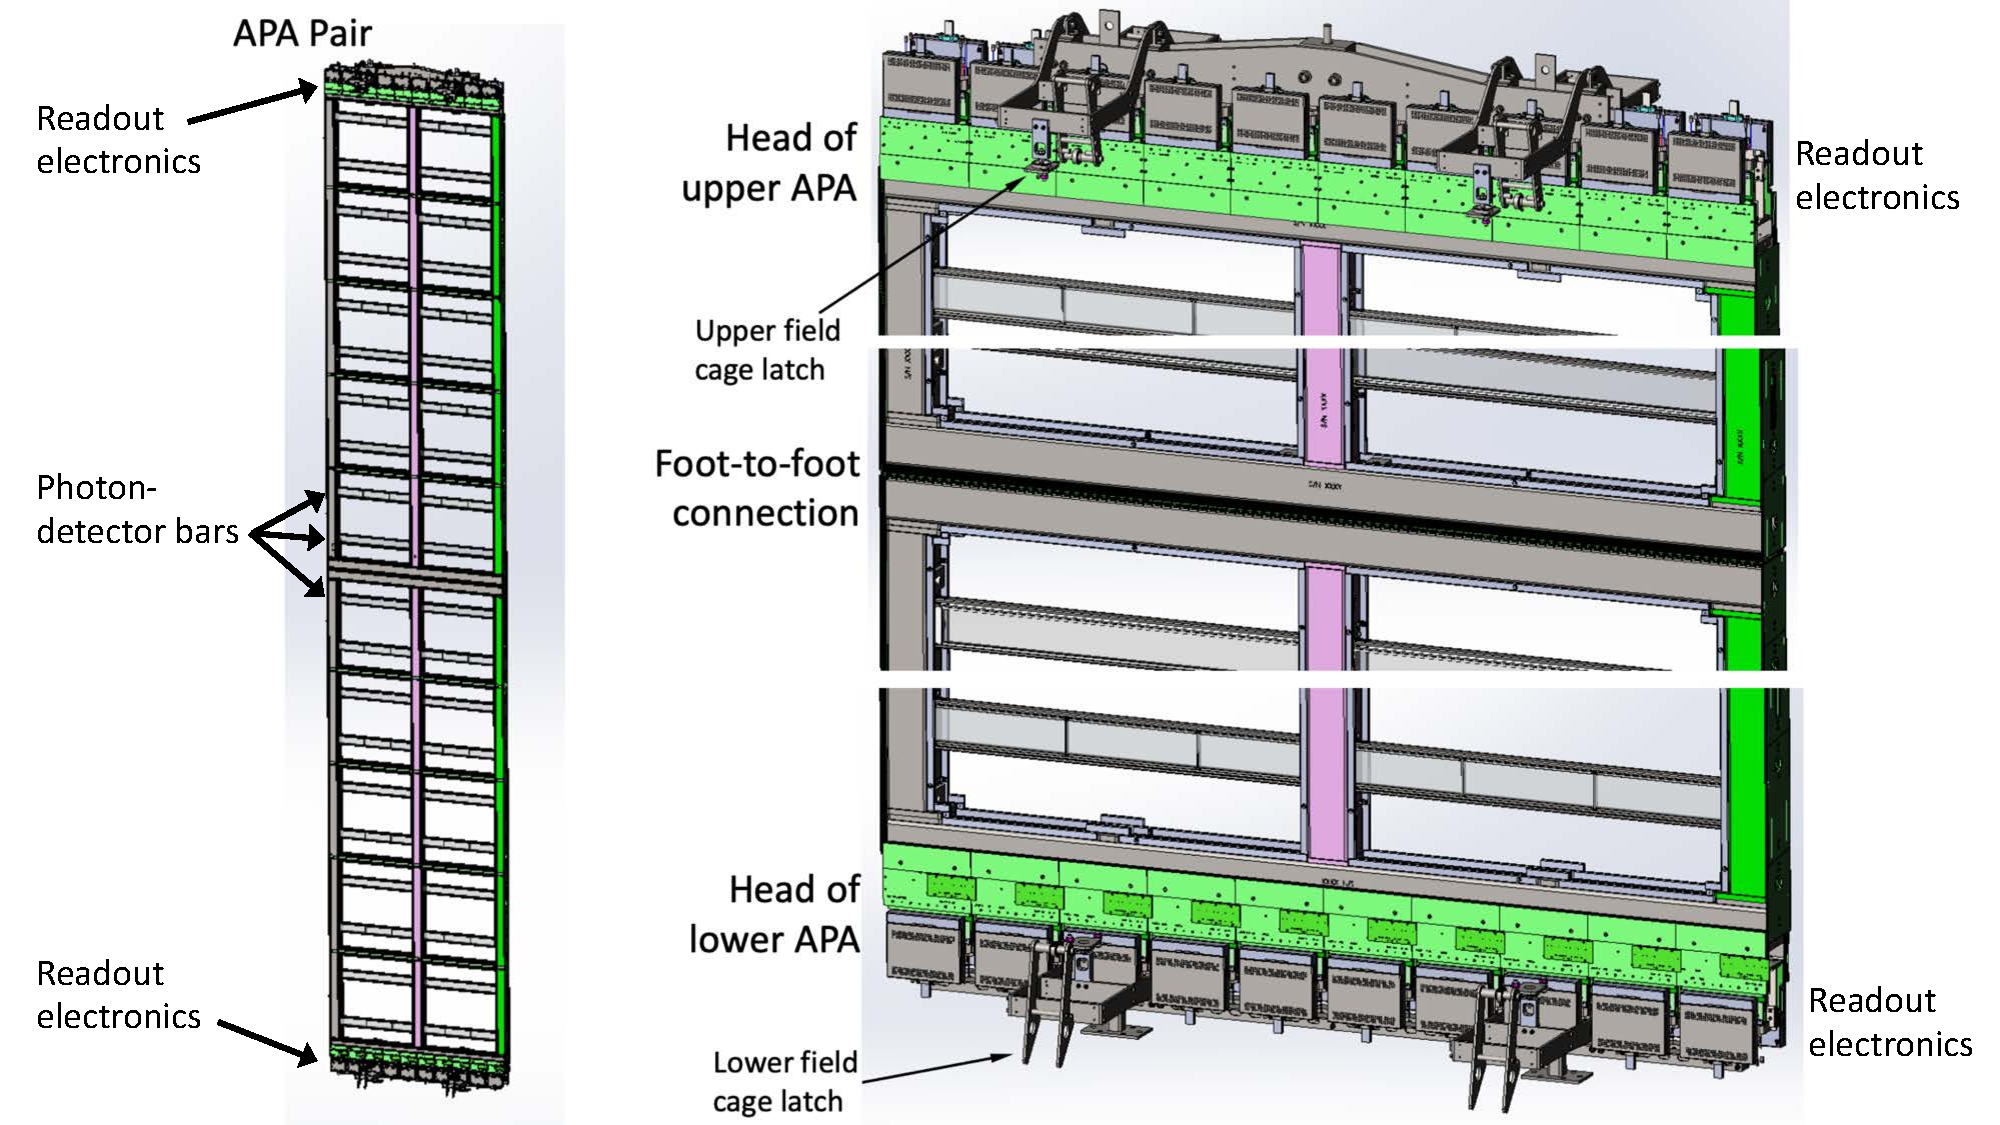
\includegraphics[width=\textwidth]{graphics/APAStack.pdf}
\end{dunefigure}

Readout electronics are attached to the \dword{apa}s; the readout happens at the top end of the top \dword{apa} and the bottom end of the bottom \dword{apa}. These front-end electronics benefit from the liquid-argon temperatures through the reduction of thermal noise. The front-end electronics shape, amplify, and digitize the signals from the induction and collection wires thanks to a series of three different types of \dword{asic} through which all signals pass. On each \dword{apa} are 20 front-end motherboards, on which the \dword{asic}s are mounted, and each motherboard processes the signals from 40 $u$, 40 $v$, and 48 $x$-layer wires. Cables from the \dword{ce} pass through feedthroughs on the roof of the cryostat; cables from the motherboards on the bottom \dword{apa} pass through the inside of the hollow \dword{apa} frames to bring them up to the top.

Once the signals from the \dword{apa}s leave the cryostat through the feedthroughs, they are passed to warm interface boards that put the signals onto \SI{10}{\giga\byte} optical fibers, ten fibres per \dword{apa}, which carry the signals to the data-acquisition system located in the \dword{cuc}, a \SI{190}{\meter} long, \SI{19.3}{\meter} wide, \SI{10.95}{\meter} high cavern adjacent to the detector caverns underground. Each \SI{10}{\kilo\tonne} module has its own, independent data-acquisition system, built around the \dword{felix} system, developed by \dword{cern}, which is responsible for triggering, buffering, and shipping data out to permanent storage above ground; when triggered, each \SI{10}{\kilo\tonne} module will provide data at a rate of up to \SI{2}{\tera\byte/\second}. This separation of data-acquisition systems allows each module to run as an independent detector to minimize any chance of a complete \dword{fd} outage. Modules can, however, provide the others with a supernova trigger signal. The data-acquisition system also provides the detector clock. A \dword{gps} \dword{pps} is used to time-stamp events, both to allow matching to the beam window and to allow time-stamping of supernova triggers. Within a \SI{10}{\kilo\tonne} module a $\SI{65}{\mega\hertz}$ master clock keeps all detector components synchronized to within \SI{1}{\nano\second}.

In addition to the ionization, charged particles passing through the argon produce approximately 24,000 scintillation photons per \si{\mega\electronvolt}. These photons are collected by devices called X-Arapucas, which are mounted on the \dword{apa}s, in between the two sets of wire layers, as shown in Figure~\ref{fig:APAStack}. There are ten X-Arapucas on each \dword{apa}, which consist of $\SI{209.2}{\cm}\times\SI{11.8}{\cm}\times\SI{2.3}{\cm}$ bars, running the full \SI{2.3}{\meter} width of the \dword{apa}. The X-Arapuca bars consist of layers of dichroic filter and wavelength-shifter that shift the \SI{126.8}{\nano\meter} light into the visible and trap these visible photons, transporting them to \dword{sipm} devices. The signals from these \dword{sipm}s are sent along cables that pass through the hollow \dword{apa} frames, up to feedthroughs in cryostat roof. The signals are then sent along \SI{10}{\giga\byte} optical fibers, one fiber per \dword{apa} (ten X-Arapuca bars), to the \dword{daq} system where the photon-detector and \dword{apa}-wire data-streams are merged.

\section{The Liquid Argon}
\label{sec:fdsp-exec-liquidargon}

The primary requirement of the liquid argon is its purity. Electronegative contaminants such as oxygen or water will absorb ionization electrons as they drift. Nitrogen contaminants will quench scintillation photons.

The target purity from electronegative contaminants in the argon is $<\!100$\,ppt O$_{2}$ equivalent, which is enough to ensure a $>\!\SI{3}{\milli\second}$ ionization-electron lifetime at our nominal \SI{500}{\volt/\centi\meter} drift voltage. This target electron lifetime means that, for an ionization event occurring near a \dword{cpa} array, there is 48\% attenuation of the ionization by the time it reaches the anode, which ensures, for these events, that we still achieve signal-to-noise ratios of $S/N>5$ for the induction planes and $S/N>10$ for the collection planes, which are necessary to perform pattern recognition and two-track separation. We have an additional requirement for electronegative impurities released into the argon by detector components of $<\!30$\,ppt, to ensure such sources of contamination are negligible compared to the contamination inherent in the argon. Data from \dword{protodune} has shown that we can exceed our target argon purity, with electron lifetimes in excess of \SI{6}{\milli\second} achieved.

Nitrogen contamination must be $<\!25$\,ppm. This is necessary to ensure we achieve our requirement of at least 0.5 photoelectrons per MeV detected for events in all parts of the detector, which in turn ensures, through the timing requirements discussed in Section~\ref{sec:fdsp-exec-pds}, that we can fiducialize nucleon decay events throughout the detector.

The argon contains a natural trace component of unstable $^{39}$Ar. This isotope undergoes $\beta$ decay, and these $\beta$-decay electron tracks, as well as the photons they produce, define the energy threshold below which we cannot trigger on low-energy physics events such as solar neutrinos without
being swamped by background. We use this $^{39}$Ar contamination to form a requirement that all other detector components must introduce negligible radioactive contamination compared to the $^{39}$Ar.

Fundamental to maintaining the argon purity is the constant flow of argon through the purification system. It is, therefore, important to understand the fluid dynamics of the argon flow within the detector to ensure no dead regions where argon can become trapped. This fluid dynamics also informs the placement of purity, temperature, and level monitors. The computational fluid dynamics, as well as the requirements for monitoring the argon and the instrumentation used to perform this monitoring, is described further in Chapter~\ref{chap:fdsp-cisc}. 


\section{Photon Detection System}
\label{sec:fdsp-exec-pds}

Compared to the ionization electrons, which can take milliseconds to drift across the drift volume, the scintillation photons are fast, arriving in nanoseconds. This fast scintillation light provides a $t_{0}$ for each event. By comparing the arrival time of ionization at the anode with this $t_{0}$, reconstruction in the drift direction becomes possible. The spatial resolution of the detector perpendicular to the drift direction is defined by the $\sim\!\SI{5}{\mm}$ wire spacing on the \dword{apa}s; a desire to achieve a comparable spatial resolution in the drift direction results in a \SI{1}{\micro\second} requirement on the timing resolution of the photon-detector system. Specifically, this requirement enables \SI{1}{\mm} position resolution for \SI{10}{\mega\electronvolt} supernova-burst events. The photon detector $t_{0}$ is also vital in fiducializing nucleon-decay events, which allows us to reject cosmic-muon-induced background events that will occur near the edges of the detector modules. We must be able to do this throughout the entire active volume with $>\!99\%$ efficiency, leading to a requirement of at least 0.5 photoelectrons per MeV detected for events in all parts of the detector, which in turn requires an effective area of $\SI{23}{\cm^{2}}$ for each photon-detector module.


\begin{dunefigure}[Photon-detector modules, mounted in an anode pane assembly.]{fig:PDModules}
{Left: a photon-detector module. Right: a photon-detector module mounted in an APA.}
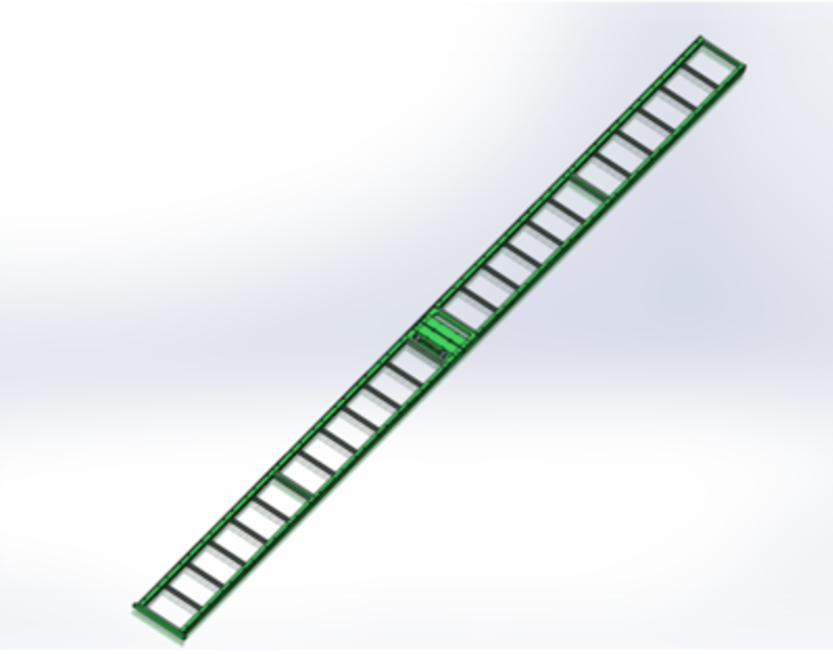
\includegraphics[width=0.49\textwidth]{PDBar.pdf}
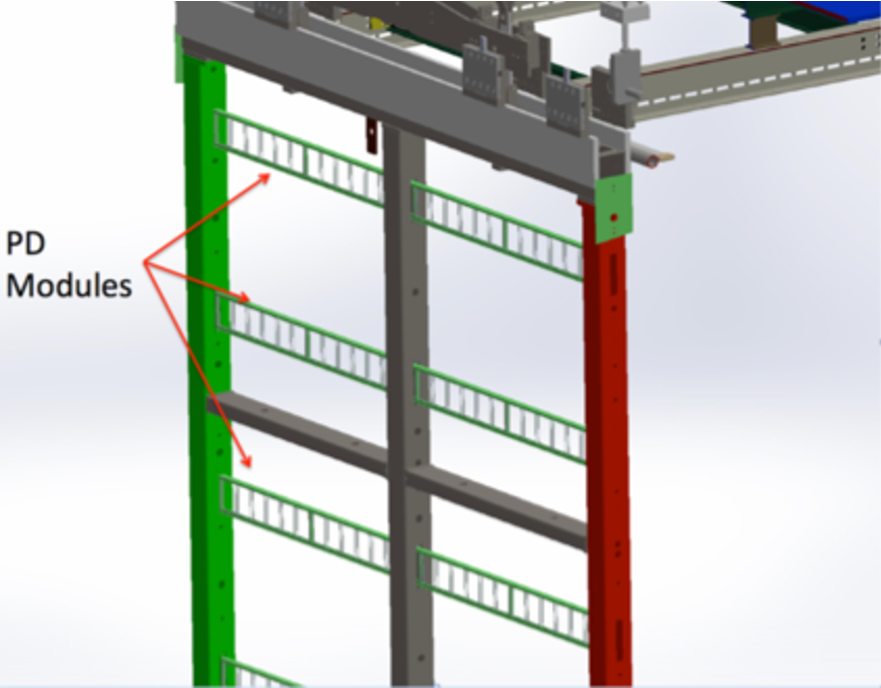
\includegraphics[width=0.49\textwidth]{PDsInAPA.pdf}
\end{dunefigure}

Photon detector modules, shown in Figure~\ref{fig:PDModules}, are $\SI{209.2}{\cm}\times\SI{11.8}{\cm}\times\SI{2.3}{\cm}$ bars, ten of which are mounted in each \dword{apa} inside the wire layers. Each bar contains 24 X-Arapuca\footnote{An arapuca is a South American bird trap, the name used here in analogy to the way the X-Arapuca devices trap photons.} cells, grouped into four supercells. An X-Arapuca cell is shown in Figure~\ref{fig:ArapucaCell}. The outer layers are dichroic filters transparent to the \SI{126.8}{\nano\meter} scintillation light. Between these filters is a \dword{wls} plate, which converts the photons into the visible spectrum; one WLS plate runs the full length of each supercell.
Visible photons emitted inside the \dword{wls} plate at an angle to the surface greater than the critical angle are transported to \dword{sipm}s at the ends of the plates. Visible photons that escape the \dword{wls} plates are reflected off the dichroic filters, which have an optical cutoff for photons with wavelengths more than \SI{400}{\nano\meter}, back into the \dword{wls} plates. 

\begin{dunefigure}[An X-Arapuca photon-detector cell.]{fig:ArapucaCell}
{Left: an X-Arapuca cell. Right: an exploded view of the X-Arapuca cell, where the blue sheet is the wavelength-shifting plate and the yellow sheets the dichroic filters.}
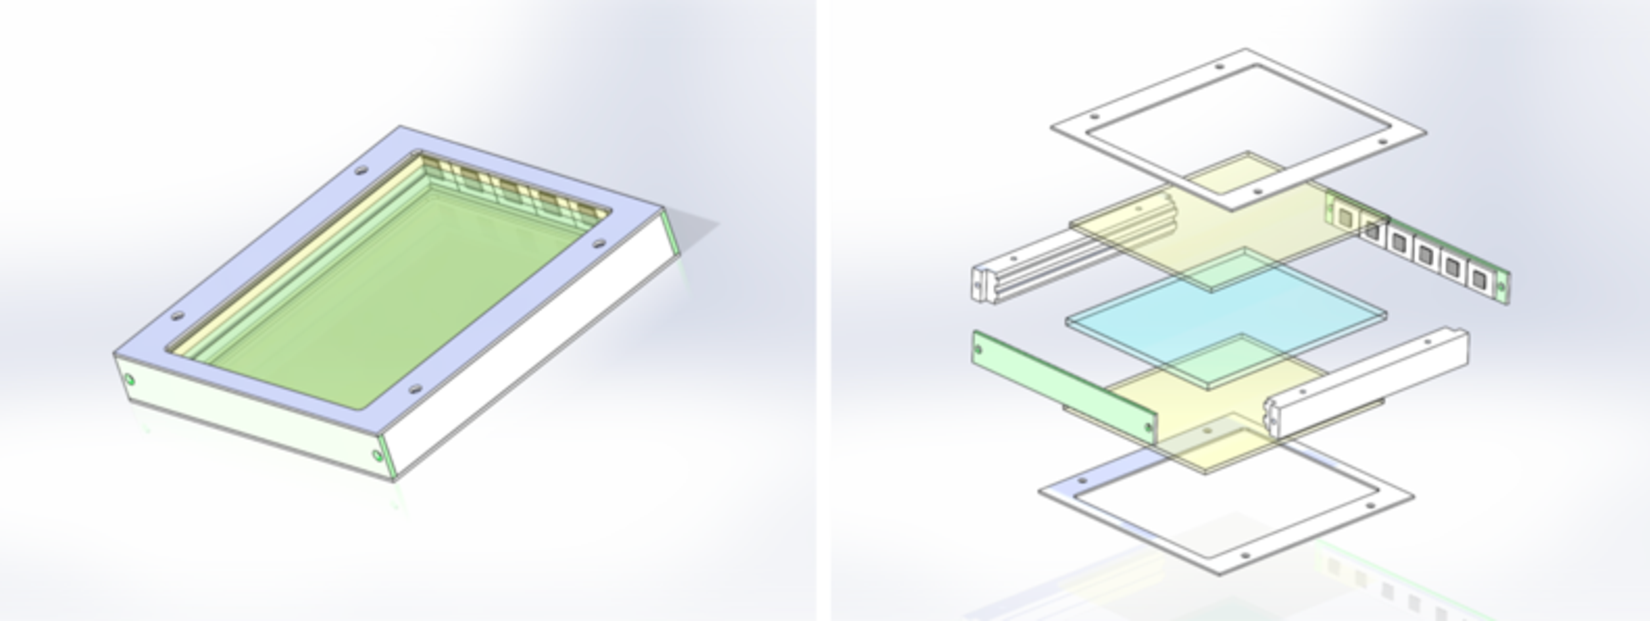
\includegraphics[width=\textwidth]{XArapuca.pdf}
\end{dunefigure}

The 48 \dword{sipm}s on each X-Arapuca module are ganged together and the signals collected by front-end electronics, mounted on the module, the design of which is inspired by the system used for the Mu2e cosmic-ray tagger, which uses commercial ultrasound \dword{asic}s. The front-end electronics define the \SI{1}{\micro\second} timing resolution of the photon-detector system.

\section{High Voltage}
\label{sec:fdsp-exec-hv}

The design voltage at which the \dword{dune} \dword{tpc} will operate is $-\SI{180}{\kilo\volt}$, corresponding to \SI{500}{\volt/\cm} across each drift volume. This voltage is a trade off. A higher voltage results in more charge collected, and hence better signal-to-noise ratio, better calorimetry, and lower detection thresholds, as well as less saturation of free charge at the point of ionization. A higher voltage, however, also reduces the amount of scintillation light produced and requires more space between the \dword{cpa}s and the \dword{fc}, reducing the fiducial volume. The \dword{protodune} experience shows that we can achieve this design voltage; nevertheless, from \dword{microboone}, we also know that a drift voltage of \SI{250}{\volt/\cm} achieves an adequate signal-to-noise ratio.

The high voltage is supplied to the \dword{cpa} arrays. Each \dword{cpa} array (two per \SI{10}{\kilo\tonne} module) has its own independent high voltage supply. These commercial high voltage devices will supply a current of \SI{0.16}{\milli\ampere} at $-\SI{180}{\kilo\volt}$. The voltage is delivered, via $\sim\!\SI{30}{\meter}$ length commercial cables, through a series of few-\si{\mega\ohm} filtering resistors that act as low-pass filters to reduce noise and thereby satisfy the ripple-voltage requirement of $<\!\SI{0.9}{\milli\volt}$ on the \dword{cpa} array, which corresponds to a requirement of $<\!100\,e{-}$ of noise injected into the \dword{tpc} by the high-voltage system. The supply unit monitors the voltage and current every \SI{300}{\milli\second}; toroids mounted on the cables are sensitive to much faster changes in current and enable responses to current changes on a timescale of \SIrange{0.1}{10}{\micro\second}.

The high voltage passes into the cryostat through a feedthrough based on the ICARUS design~\cite{Icarus-T600}, the stainless steel conductor of which mates with the \dword{cpa} array via a spring-loaded feedthrough.
When at $-\SI{180}{\kilo\volt}$, each \dword{cpa} array stores \SI{400}{\joule} of energy, so the \dword{cpa}s must have at least $\SI{1}{\mega\ohm/\cm^{2}}$ resistance to prevent damage if the field is quenched. The \dword{cpa}, one of which is shown in Figure~\ref{fig:CPA}, is a $\SI{1.2}{\meter}\times\SI{2}{\meter}$ planar unit, each side of which is a \SI{3}{\mm} thick FR-4 sheet, onto which is laminated a thin layer of carbon-impregnated Kapton that forms the resistive cathodic plane.

\begin{dunefigure}[A cathode plane assembly.]{fig:CPA}
{A cathode plane assembly.}
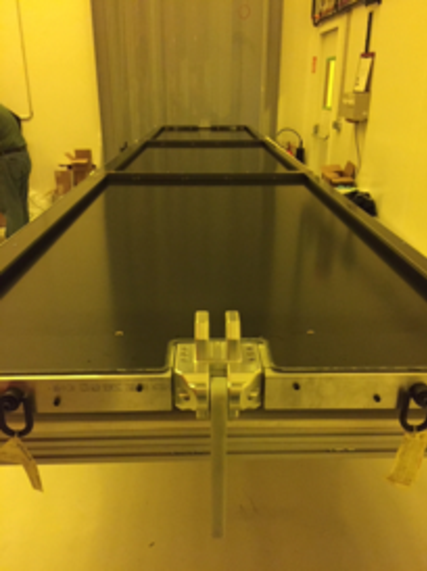
\includegraphics[width=0.35\textwidth]{CPA.pdf}
\end{dunefigure}

The field must be uniform throughout the active \dword{tpc} volume to within 1\%, and this is achieved by an \dword{fc} that surrounds the drift volumes. The \dword{fc} is built from field-shaping aluminum profiles, terminated with \SI{6}{\mm} thick ultra-high molecular-weight polyethylene caps (see Figure~\ref{fig:FieldCage}). All surfaces on these profiles must be smooth to keep local fields below \SI{30}{\kilo\volt/\cm}, a requirement that reduces the possibility of voltage breakdowns in the argon; the shape of the profiles chosen leads to a maximum local field near the surface of the \dword{fc} of $\sim\!\SI{12}{\kilo\volt/\cm}$. The aluminum profiles are connected together via a resistive divider chain; between each profile, two \SI{5}{\giga\ohm} resistors, arranged in parallel, provide a \SI{2500}{\mega\ohm} resistance to create a nominal \SI{3}{\kilo\volt} drop.

\begin{dunefigure}[A section of the field cage.]{fig:FieldCage}
{A section of the field cage, showing the extruded aluminium field-shaping profiles.}
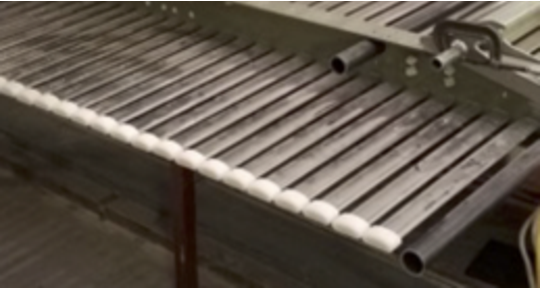
\includegraphics[width=0.5\textwidth]{FieldCage.pdf}
\end{dunefigure}

\section{Anode Planes}
\label{sec:fdsp-exec-apas}

The \dword{apa}s are $\SI{6}{\meter}\times\SI{2.3}{\meter}$ planes that form the three anodic walls of the \dword{tpc}: two along the edges and one down the middle, as shown in Figure~\ref{fig:DUNESchematic}. An \dword{apa} is shown in Figure~\ref{fig:APA}. In the \dword{fd}, the \dword{apa}s are mounted in pairs, in portrait orientation, one above another, with the head end of the top \dword{apa} at the top of the detector and the head end of the bottom \dword{apa} at the bottom of the detector.

\begin{dunefigure}[An anode plane assembly.]{fig:APA}
{Top: a schematic of an anode plane assembly. Bottom: a ProtoDUNE anode plane assembly. The right-hand end of the APA as shown in this picture is the head end, onto which the cold electronics is mounted (the blue boxes in the upper picture). }
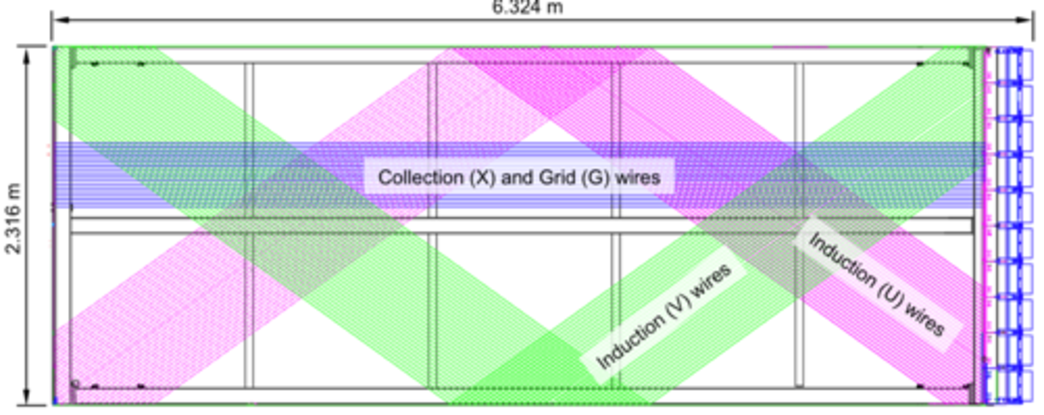
\includegraphics[width=0.7\textwidth]{APASchematic.pdf}
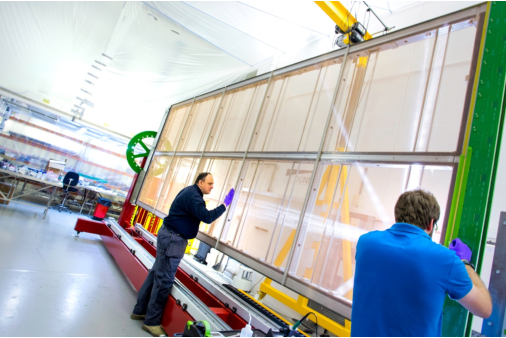
\includegraphics[width=0.6\textwidth]{RealAPA.pdf}
\end{dunefigure}

The basic building block of the \dword{apa} is the $\SI{6}{\meter}\times\SI{2.3}{\meter}$ steel frame that can be seen outlined in Figure~\ref{fig:APA}, consisting of three long sections, a head shaft onto which the \dword{ce} is mounted, a foot shaft, and four thinner cross-braces. The two outer long sections are $4\,\mathrm{inch}\times 4\,\mathrm{inch}$ square-profile steel tubes through which run the photon detector cables and the \dword{ce} cables from the bottom \dword{apa} of a pair. The photon detectors are mounted into the \dword{apa}s, after production, through slots in these long sections.

Mounted directly onto both sides of the \dword{apa} frame is a grounding mesh, which ensures any ionization produced inside the \dword{apa} cannot cause signals on the active wire layers. Around this mesh are wound the four wire layers, consisting of \SI{150}{\micro\meter} diameter copper-beryllium wire. The inside layer is the collection layer, called the $x$-layer, the 960 wires of which run parallel to the long axis of the \dword{apa}. Next are the two induction layers, the $u$- and $v$-layers, each with 800 wires at \SI{35.7}{\degree} to the long axis. Finally, the uninstrumented shielding layer, the $g$-layer, has 960 wires running parallel to the $x$-layer wires; this layer shields the three active layers from long-range induction effects. The wire spacing on each layer is close to \SI{5}{\mm}, and the inter-plane spacing is \SI{4.75}{\mm}. The $\sim\!\SI{5}{\mm}$ spacing on each plane defines the spatial resolution of the \dword{apa}; it is wide enough to keep readout costs low and signal-to-noise high, but small enough to enable reconstruction of short tracks such as few-\si{\cm} kaon tracks from proton-decay events. The tolerance both on the wire spacing in the plane and on the plane-to-plane spacing is \SI{0.5}{\mm}; this is most important in the plane-to-plane direction where the spacing ensures that the induction planes remain transparent to the drifting charge.

Around the four sides of the \dword{apa} are printed circuit boards called geometry boards to which the wires are soldered, so-called because these boards define the wire spacing in all dimensions. These boards, shown in Figure~\ref{fig:GeometryBoardsAndCombs}, consist only of pads and traces: no active components. At the head end, these boards lie flat in the plane of the \dword{apa}, and the wires are terminated onto these boards for readout. On the remaining three sides, the boards sit on the sides of the \dword{apa}, perpendicular to the wire planes, and control the wrapping of the wires around the \dword{apa}. These wrap boards have insulating pins on their edges, around which the wires are wrapped, to set the wire spacing. At the head end, additional active boards are installed after all wires are wound: $g$-bias boards provide the necessary capacitance to the $g$-layer and a resistor to provide the bias voltage; $CR$-boards provide the interface between the $x$ and $u$ layers and the \dword{ce}, resistors providing the bias voltages and capacitors providing DC blocking. Relative to the ground, the four wire layers are biased to \SI{820}{\volt} ($x$-layer), \SI{0}{\volt} ($v$-layer), \SI{-370}{\volt} ($u$-layer), and \SI{-665}{\volt} ($g$-layer). To maintain the wire spacing across the \dword{apa}, wire-support combs, also shown in Figure~\ref{fig:GeometryBoardsAndCombs}, run along the four cross-braces across the short dimension of the \dword{apa}.

\begin{dunefigure}[Geometry boards and wire-support combs on an anode plane assembly.]{fig:GeometryBoardsAndCombs}
{Left: geometry boards, showing the head-end boards face-on and the wrap boards along the bottom. Back plastic teeth are visible on the edges of the wrap boards. Right: wire-support combs.}
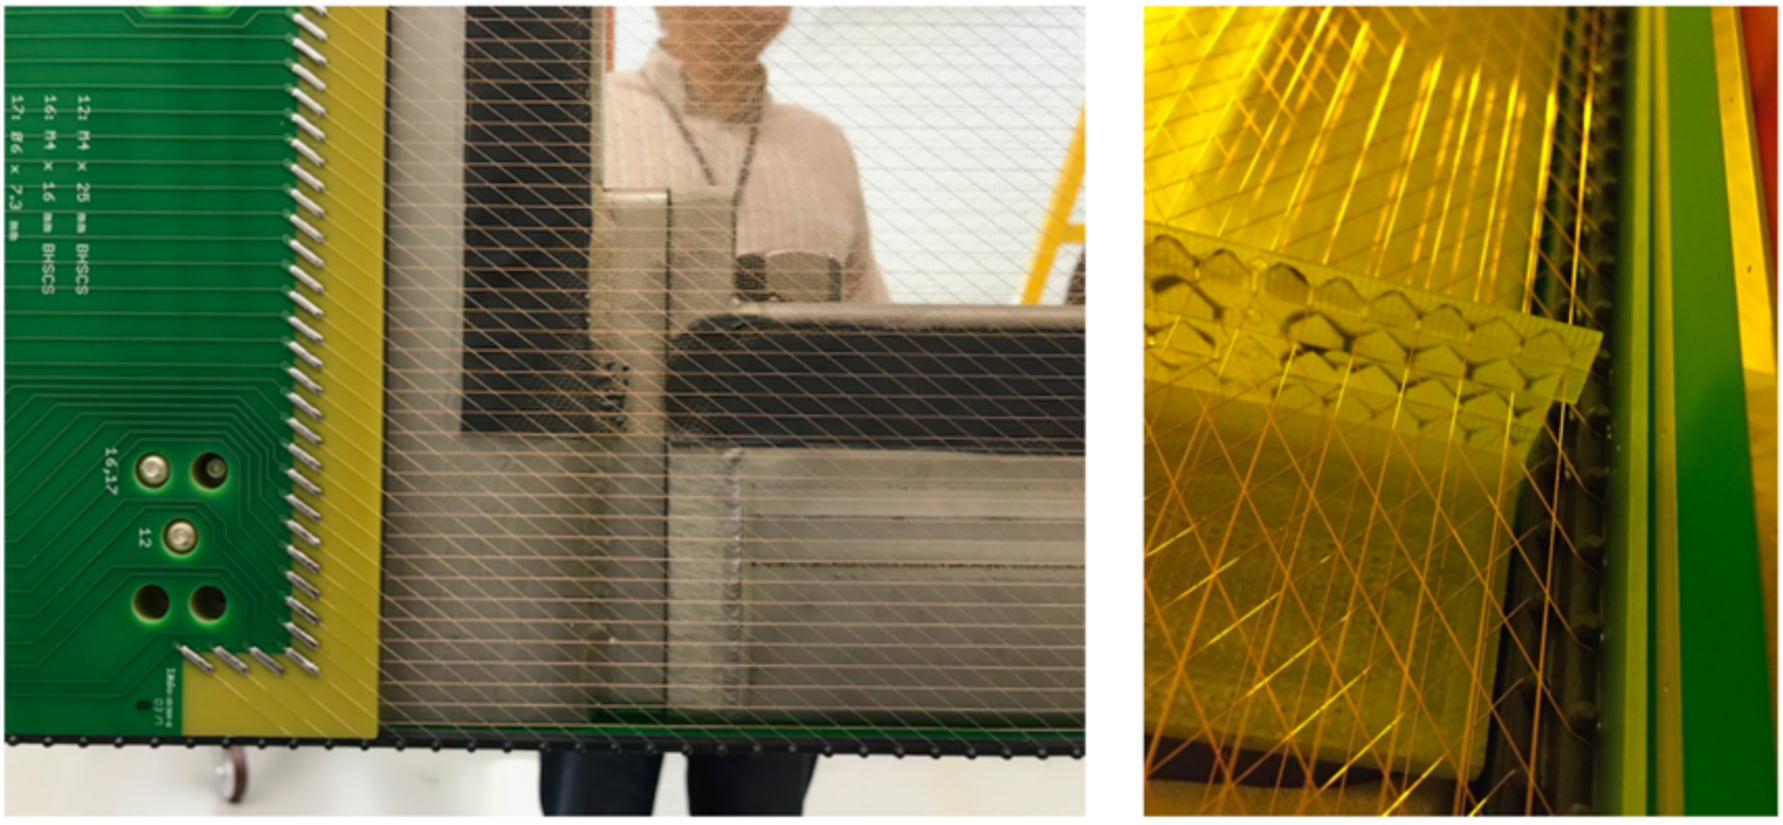
\includegraphics[width=\textwidth]{GeometryBoardsAndCombs.pdf}
\end{dunefigure}

In the \dword{fd}, \dword{apa}s are hung in pairs, one above another, the bottom \dword{apa} hanging from the top \dword{apa}, as was shown in Figure~\ref{fig:APAStack}. Each \dword{apa} must be electrically isolated from all its neighbors, so the mechanical linkages are made using parts made from G10.

\section{Electronics}
\label{sec:fdsp-exec-electronics}

The job of the readout electronics is to send out of the cryostat digitized waveforms from the \dword{apa} wires. To enable us to look at low-energy particles, we aim to keep noise to below $1000\,e^{-}$ per channel, which should be compared to the $20k$--$30k\,e^{-}$ per channel from a minimum-ionizing particle. For large signals, we require a linear response up to $500,000\,e^{-}$, which ensures that fewer than 10\% of beam events experience saturation. This can be achieved using 12\, \dword{adc} bits. In addition, the electronics are designed with a front-end peaking time of \SI{1}{\micro\second}, which matches the time for the electrons to drift between wires planes on the \dword{apa}; this then leads to a design sampling frequency of \SI{2}{\mega\hertz}.

The digitization electronics are mounted on the head ends of the \dword{apa}s in the liquid argon and are therefore referred to as cold electronics. The low temperatures reduce thermal noise. Figure~\ref{fig:ElectronicsBlockDiagram} shows a block diagram of the front-end motherboards mounted on the \dword{apa}s. Each \dword{apa} is instrumented with 20 front-end motherboards, each of which takes the signals from 40 $u$-layer wires, 40 $v$-layer wires, and 48 $x$-layer wires. The signals all pass through a series of three \dword{asic}s. The first \dword{asic}, the front-end \dword{asic}, shapes and amplifies the signals. The next \dword{asic}, the \dword{adc} \dword{asic}, performs the analogue-to-digital conversion. Finally, a \dword{coldata} \dword{asic} merges the datastreams from the preceding \dword{asic}s for transmission to the outside world; this \dword{coldata} \dword{asic} also controls the front-end motherboard and facilitates communications between the motherboard and the outside world.

\begin{dunefigure}[A block diagram of the anode-plane readout electronics.]{fig:ElectronicsBlockDiagram}
{A block diagram of the readout electronics mounted on the APAs. The FEMB is the front-end motherboard.}
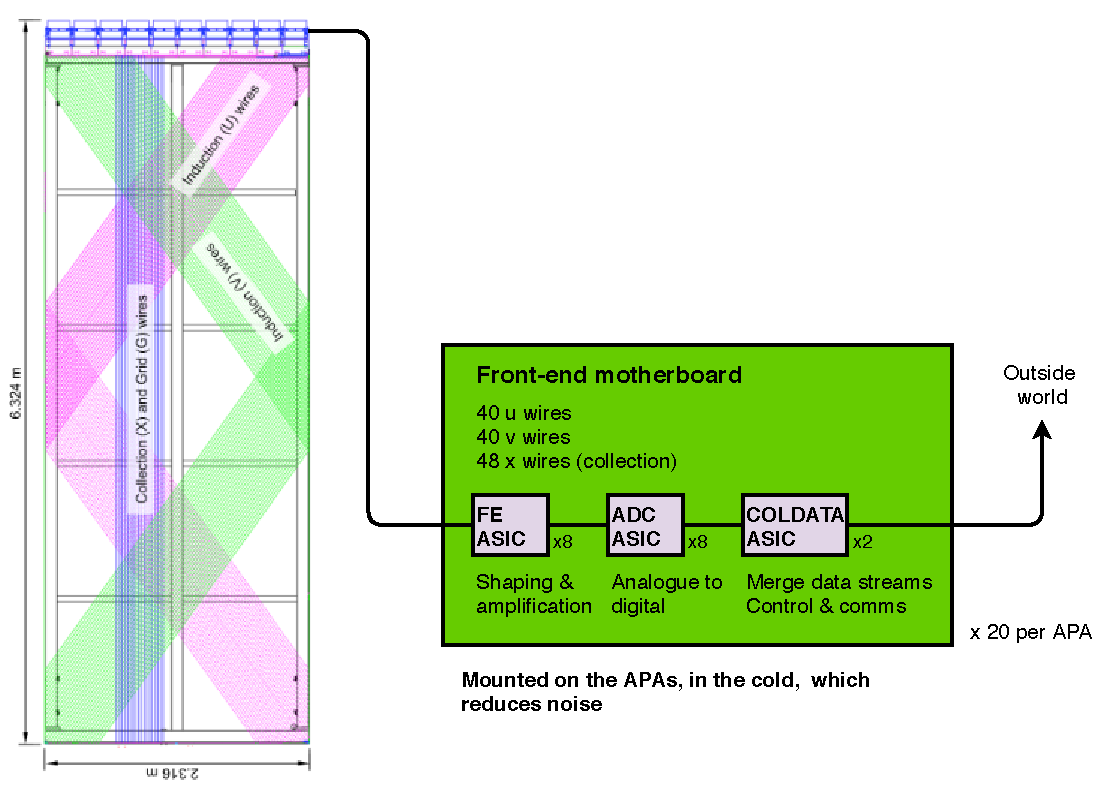
\includegraphics[width=0.8\textwidth]{ElectronicsBlockDiagram.pdf}
\end{dunefigure}

Once the data has passed out of the cryostat through feedthroughs in the roof, it is passed to warm interface boards, which transmit the signals to the \dword{daq} system along \SI{10}{\giga\byte/\second} optical fibers. These warm interface boards also transmit the clock and control signals and the low-voltage power back to the front-end motherboards.

\section{Data Acquisition}
\label{sec:fdsp-exec-daq}

The \dword{daq} is located underground, in the \dword{cuc}, adjacent to the main detector caverns. The \dword{daq} is based on the \dword{felix} system designed at \dword{cern} and used for the LHC \fixme{This abbreviation (LHC) is not in the common glossary.} experiments. Each \SI{10}{\kilo\tonne} module has its own independent \dword{daq} system. The \dword{daq} must independently trigger the \dword{tpc} readout for all event types, including beam events, nucleon-decay events, and supernova bursts.

The supernova burst provides the \dword{daq} with the greatest challenge. Here, the \dword{daq} must, with zero dead-time, trigger on interactions below \SI{100}{\mega\electronvolt} spaced over many seconds, throughout the detector volume. The target for doing this is $>\!90\%$ efficiency for each \SI{10}{\kilo\tonne} module for supernovae within \SI{100}{\kilo\parsec}; once triggered, a module will then send a trigger signal through to the other three modules. The \dword{daq} must then handle the immense data-rate involved: the entire detector must be read out for up to \SI{100}{\second}, including a \SI{4}{\second} pre-trigger window; the full data-rate from a module can be as high as \SI{2}{\tera\byte/\second}. For beam events and nucleon-decay events, the problem is much simpler because only a localized part of the detector around the event need be read out, and the read-out window only needs to be approximately the length of a drift window: around \SI{30}{\milli\second}.

The 150 \dword{apa}s from each \SI{10}{\kilo\tonne} module are processed by 75 \dword{felix} boards. The photon detectors from the module will have a lower data rate, and so will be processed by six to eight additional \dword{felix} boards. Each \dword{felix} board sits below ground in its own host server and talks to a data-selection server that may be either above or below ground. The data is finally transferred to \dword{fermilab} over a network; our goal is to achieve a data rate to tape of less than \SI{30}{\peta\byte/\year}.

The \dword{daq} must also provide the system clock that keeps the detector components synchronized and timestamps all the data. The timestamp derives from a \dword{gps} \dword{pps} that is fed into the \dword{daq} with \SI{1}{\micro\second} precision, adequate precision to timestamp beam and supernova events. To provide the finer synchronization between detector components, a \SI{10}{\mega\hertz} reference clock drives the module's \SI{65}{\mega\hertz} masterclock, which is fanned out to all detector components, providing an overall synchronization to a precision of \SI{1}{\nano\second}.

\section{Calibration}
\label{sec:fdsp-exec-calibration}

The challenge of calibrating the \dword{dune} \dword{fd} is the challenge of controling the response of a huge cryogenic detector over a period of decades, a challenge amplified by the detector's location deep underground and therefore shielded from the cosmic muons used as standard candles by previous \dword{lartpc}s.

To achieve our $\mathcal{O}(\si{\giga\electronvolt})$ oscillation and nucleon decay physics goals, we must know our fiducial volume, and determine vertex locations, to 1--2\%; understand the \nue event rate to 2\%; and control our lepton and hadron energy scales to 1\% and 3\%, respectively. At the $\mathcal{O}(\si{\mega\electronvolt})$ scale our physics requirements are driven by our goal of identifying, and measuring the spectral structure of, a supernova neutrino burst; here, we must achieve a 20--30\% energy resolution, understand our event timing to the \SI{1}{\micro\second} level, and measure our trigger efficiency and our levels of radiological background. These are all high-level calibration requirements, but the underlying detector parameters that we are characterising are parameters such as $\mathrm{d}E/\mathrm{d}x$, ionisation electron lifetimes and drift patterns, scintillation light output and detection, electric field maps, timing precision, \dword{tpc} alignment, and the behaviour (noise, gain, cross-talk, linearity, etc.) of electronics channels.

The tools available to us for calibration include the \dword{lbnf} beam, cosmic rays, radiological backgrounds, and dedicated calibration devices that will be installed in the detector. At the lowest energies, we have both intrinsic and deployable radioactive and neutron sources; in particular the natural $^{39}$Ar component of the \dword{lar} will act as a standard candle. In the \SIrange{10}{100}{\mega\electronvolt} energy range we will use Michel electrons, photons from $\pi^{0}$ decay, stopping protons and both stopping and through-going muons. We will also have built-in lasers, purity monitors and thermometers, and the ability to inject charge into the readout electronics. Finally, data from the \dword{protodune} detector will be invaluable in understanding the response and particle-identification capabilities of the \dword{fd}.

Once the first \SI{10}{\kilo\tonne} module is switched on, there will be a period of years before \dword{lbnf} beam sources are available as calibration tools. In this time, cosmic muons will be available, but the low rate of these means that it will take months to years to build up the necessary statistics for calibration. The total cosmic muon rate for each \SI{10}{\kilo\tonne} module is $1.3\times 10^{6}$ per year. However, for calibrations such as \dword{apa} alignment, the typical rate of useful muons is 3000--4000 per APA gap per year. For energy-scale calibrations, stopping cosmic muons are the most relevant and here the rate is 11000 per \SI{10}{\kilo\tonne} module per year. Therefore the earliest calibrations will come from dedicated calibration hardware systems and radiological sources.

A \SI{266}{\nano\meter} laser will be used to ionise the argon, and this can be used to map the electric field and to make early measurements of \dword{apa} alignment. The laser system will be used throughout the lifetime of the detector to measure the gradual changes in the electric field map as positive ions accumulate and flow around the detector. The natural $^{39}$Ar $\beta$-decay rate in commercial argon is $\sim\!\SI{1}{\becquerel\,\kilo\gram^{-1}}$. With an end-point energy of \SI{565}{\kilo\electronvolt}, close to the energy deposited on a single wire by a \dword{mip}, the reconstructed energy spectrum and observed signal shapes can be used to measure the spacial and temporal variation of electron lifetime, the wire-to-wire response variations and the diffusion of ionisation. Other radioactive sources, including a pulsed neutron source and a radioactive source deployment system, are also under consideration.

Over time, the \dword{fd} calibration programme will evolve as statistics from the cosmic rays and the \dword{lbnf} beam amass and add to the information gained from the calibration hardware systems, many of which are still under development. These numerous calibration tools will work alongside the detector monitoring system, the computational fluid dynamics models of the argon flow, and \dword{protodune} data to give us a detailed understanding of the \dword{fd} response right across the \dword{dune} physics programme.


\section{Conclusion}
\label{sec:fdsp-exec-conclusion}

This executive summary has described the design of the \SI{10}{\kilo\tonne} \dword{sp} \dword{lartpc} modules of the \dword{dune} \dword{fd}, explaining how key design choices have been made to ensure we can achieve our primary physics goals. The chapters that follow go into significantly more detail about the design of the \dword{sp} \dword{fd} modules. In addition to describing the design and requirements, these chapters include details on construction and \dword{qc} procedures, and describe how the design has been validated and informed by \dword{protodune}.

A major factor in realising the \dword{dune} \dword{sp} modules is the challenge of transporting all the detector components \SI{1500}{\meter} down the Ross shaft to the \SI{4850}{\foot} level of \dword{surf}. They must then be transferred to the \SI{144.5}{\meter} long, \SI{19.8}{\meter} wide and \SI{27.95}{\meter} high detector caverns, the bottom of which are at the \SI{4910}{\foot} level. Within the detector caverns, the components must be installed into the cryostats, with outer dimensions of \SI{62}{\meter} length, \SI{19}{\meter} width and \SI{18}{\meter} height, through a \dword{tco} at one end. Once the \dword{tco} is closed up, final installation takes place inside the cryostat, with access and equipment-removal through the roof, before the final sealing of the cryostat takes place and the argon fill can begin.

Throughout the installation process, safety is the paramount consideration: safety both of personnel and of the detector components. Once the detectors are taking data, safety is still the priority with the \dword{ddss} monitoring for argon level drops, water leaks and smoke. A detailed detector and cavern grounding scheme has been developed that not only guards against ground loops, but also ensures that any power faults are safely shunted to the facility ground.

The detector design ensures that we can achieve our key physics goals of searching for leptonic $CP$ violation, proton decay and neutrinos from supernova bursts. This is coupled with construction, \dword{qa}, \dword{qc} and installation procedures that ensure safe installation of high-quality hardware into the cryostats. Ongoing detector monitoring and a fully integrated \dword{ddss} then ensure that the detector modules will continue to take high-quality data over a number of decades, leading to an extensive output of world-class physics publications.

